%  Typ dokumentu - článek, prezentace aj.
\documentclass[english]{article}

%  Nastaví vstupní a výstupní kódování znaků (encoding) a lokalizace
\usepackage[T1]{fontenc}
\usepackage[utf8]{inputenc}
\usepackage[english,czech]{babel}
\usepackage{icomma}
\usepackage{lmodern}

%  Formát papíru a odsazení od jeho okrajů
\usepackage[letterpaper]{geometry}
\geometry{verbose,tmargin=1.5cm,bmargin=2cm,lmargin=2cm,rmargin=2cm}

%  Umožňuje pracovat s grafikou
\usepackage{graphicx}

%  Automaticky odsadí i první paragraf v každé sekci
\usepackage{indentfirst}

%  Umožňuje rozdělovat obsah na více sloupců
\usepackage{multicol}

%  Umožňuje používat hypertextové odkazy, nastavuje jejich barvu a
%  vlastnosti
\usepackage[unicode]{hyperref}
\hypersetup{
colorlinks=true, citecolor=blue, filecolor=blue, linkcolor=blue,
urlcolor=blue
}

%  Umožnění odstranění italiky u jednotek
\newcommand{\unit}[1]{\mathrm{#1}}

%  Formátování stránek, empty = odstraní číslování
% \pagestyle{empty}

%  Řádkování
\linespread{1.2}

%  Lepší zobrazování matematiky (rozšíření sum o \limits atd.)
\everymath{\displaystyle}

% Umožní psát přes \mathbb{N/R/Q/..} množiny čísel
\usepackage{amssymb}

%  Velikost fontu matematických výrazů v dokumentu lze pro danou
% základního fontu dokumentu upravit pomocí:
% \DeclareMathSizes{X}{Y}{Z}{U} kde:
% X je velikost fontu v dokumentu, pro kterou se matematika upraví
% Y je standartní velikost fontu matematiky
% Z je velikost fontu zmenšených (vnořených výrazů)
% U je velikost fontu ještě více zmenšených (vnořených výrazů).
\DeclareMathSizes{10}{10.5}{9}{9}

%  Nastaví autora, název, datum, skupinu měření apod. (můj vlastní
% příkaz, umožní znovu-použití v dokumentu)
\newcommand{\Author}{David Roesel}
\newcommand{\Coauthor}{Tereza Schönfeldová}
\newcommand{\Institute}{FJFI ČVUT v Praze}
\newcommand{\Subject}{FYZIKÁLNÍ PRAKTIKUM I}
\newcommand{\Group}{7}
\newcommand{\Circle}{ZS 5}
\newcommand{\Title}{Úloha \#10 \\Harmonické oscilace, Pohlovo torzní kyvadlo}
\newcommand{\Date}{25.10.2013}

% Začátek dokumentu - Formátování na výstup
\begin{document}

% Interní proměnné, možno zobrazovat u prezentací, používají se při
% generování pomocí \titlepage apod.
\author{\Author}
\title{\Title}
\date{\Date}

%  Lokalizace některých názvů do češtiny
\renewcommand{\figurename}{Obr.}
\renewcommand{\tablename}{Tab.}
\renewcommand{\refname}{Reference}

% --- Hlavička dokumentu -----------------------------------------------

\setlength{\parindent}{0cm}
\begin{multicols}{2}
\textbf{\Subject \\
        \Institute \\[0.1cm]
%\large  \Title \\[0.5cm]
\Title \\[0.5cm]
}
\begin{tabular}{rlrl}
\large Datum měření: & \Date & \large Skupina: & \Group \\
\large Jméno: & \Author & \large Kroužek:  & \Circle\\
\large Spolupracovala: & \Coauthor &\large Klasifikace:\\
\end{tabular}

\begin{flushright}

\includegraphics[scale=0.28]{../../_meta/fjfi_standart.pdf}
\hspace{0.2cm}
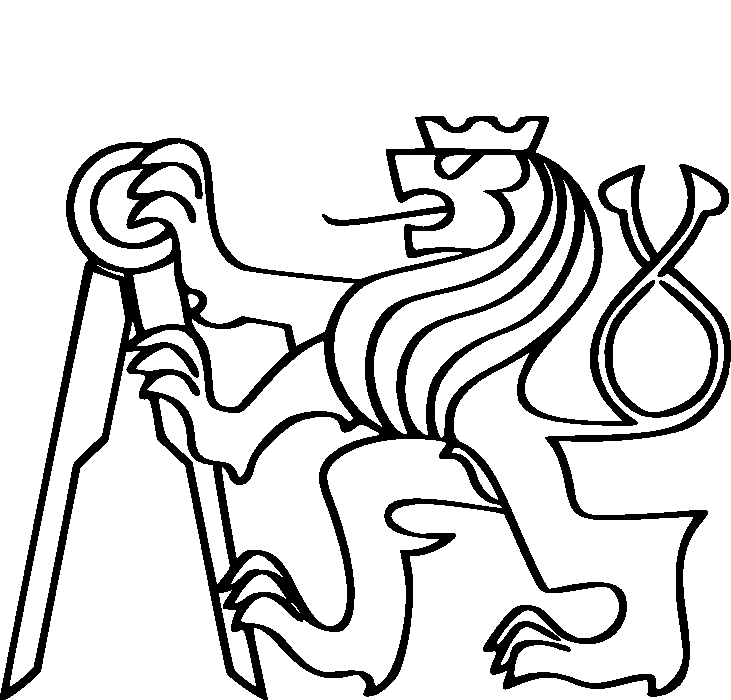
\includegraphics[scale=0.28]{../../_meta/cvut_standart.pdf}
\end{flushright}
\end{multicols}
\hrule
\vspace{0.5cm}

% ----------------------------------------------------------------------


% --- Tělo dokumentu ---------------------------------------------------

% Ocitovat markovu hlavičku
% Zeptat se na značky přístrojů

\setlength{\parindent}{0.5cm}
\part{Lineární harmonický oscilátor}

\section{Pracovní úkoly}
	\begin{enumerate}
	\item Změřte tuhost pružiny statickou metodou a vypočtěte vlastní úhlovou frekvenci pro dvě různá závaží.
	\item Změřte časový průběh tlumených kmitů pro dvě závaží, ověřte platnost rovnice (14) v \cite{bib:zadani_1} proložením dat a z parametrů proložení vypočtěte vlastní frekvenci volného oscilátoru.
	\item Změřte závislost amplitudy vynucených kmitů na frekvenci vnější síly v okolí rezonance pro dvě závaží a proložením dat ověřte platnost vztahu (19) v \cite{bib:zadani_1}, z parametrů proložení vypočtěte vlastní frekvenci volného oscilátoru.
	\item Porovnejte výsledky vlastní frekvence ze všech tří předchozích úkolů.
	\end{enumerate}

\section{Vypracování}

\subsection{Použité přístroje}
	Experimentální stojan s pružinou, závažím a motorkem, tlumící magnety, rotační pohybové senory Pasco, sada závaží, regulovatelný zdroj 0-20 V, PC, program \emph{DataStudio} a \emph{GNUplot}, laserový otáčkoměr.

\subsection{Teoretický úvod}
	\subsubsection{Potenciál harmonického oscilátoru}
		Potenciál lineárního harmonického oscilátoru má tvar 
		\begin{equation} \label{eq:potencial_oscilatoru}
		U(x) = \frac{1}{2}kx^2.
		\end{equation}
		V našem případě půjde o pružinu se zavěšeným závažím a konstanta $k$ tak bude odpovídat tuhosti pružiny v Hookově zákonu
		\begin{equation} \label{eq:hookuv_zakon}
		F = -kx,
		\end{equation}
		kde $x$ je prodloužení pružiny vyvolané působením síly $F$.
	
	\subsubsection{Netlumené kmity}
		Pohybová rovnice pro těleso o hmotnosti $m$ příslušná potenciálu (\ref{eq:potencial_oscilatoru}) má tvar 
		\begin{equation} \label{eq:pohybova_rovnice_lho}
		\ddot{x} + \omega^2 x = 0,\qquad \omega = \sqrt{\frac{k}{m}}.
		\end{equation}
		Obecné řešení této rovnice je v určitém tvaru 
		\begin{equation}
		x(t) = a\cdot \cos( \omega t + \alpha),
		\end{equation}
		kde $a$ je amplituda oscilací, $\alpha$ počáteční fáze a $\omega$ úhlová frekvence. V případě parabolického potenciálu (\ref{eq:potencial_oscilatoru}) úhlová frekvence nezávisí na počátečních podmínkách a je dána výhradně vlastnostmi oscilátoru.
\iffalse	
	\subsubsection{Vynucené kmity}
		Pokud na harmonický oscilátor působí časově proměnná vnější síla $F(t)$ a , příslušná pohybová rovnice nabývá tvar
		\begin{equation}
		\ddot{x} + \omega^2 x = \frac{F(t)}{m}.
		\end{equation}
		Uvažujeme-li periodickou budící sílu s frekvencí $\gamma$
		\begin{equation}
		F(t) = f \cos(\gamma t + \beta),
		\end{equation}
		pak pro ni najdeme partikulární řešení ve tvaru 
		\begin{equation}
		x = b \cos(\gamma t + \beta), \qquad b = \frac{f}{m}\frac{1}{\omega^2 - \gamma^2}.
		\end{equation}
		Sečtením a dosazením pak pro úplné řešení dostáváme 
		\begin{equation}
		x(t) = \tilde{a} \cos(\omega t + \alpha) + \frac{f}{m}\frac{1}{\omega^2 - \gamma^2} \left[ \cos( \gamma t + \beta ) - \cos( \omega t + \beta ) \right],
		\end{equation}
		kde si pro případ rezonance $ \gamma \rightarrow \omega$ vypomůžeme limitou a dostaneme
		\begin{equation}
		x(t) = \tilde{a} \cos(\omega t + \alpha) + t\frac{f}{2 m \omega} \sin( \omega t + \beta ).
		\end{equation}
		Z čehož vidíme, že amplituda v tomto případě roste s časem lineárně.
\fi		
		\subsubsection{Tlumené kmity}
		Z platnosti základní pohybové rovnice pro tření, zavedení dekrementu útlumu $\delta$ a frekvence volného oscilátoru bez tření $\omega_0$ podle vztahů
		\begin{equation}
		m \ddot{x} = -kx - h \dot{x}, \qquad 2\delta = \frac{h}{m}, \qquad \omega_0^2 = \frac{k}{m},
		\end{equation}
		dostaneme pohybovou rovnici tlumeného oscilátoru ve tvaru
		\begin{equation} \label{eq:pohyb_rovnice_tlumene_kmity}
		\ddot{x} = 2 \delta \dot{x} + \omega_0^2 x = 0.
		\end{equation}	
		Obecné řešení této rovnice má tvar
		\begin{equation}
		x(t) = c_1 \mathrm{e}^{\lambda_1 t}  + c_2 \mathrm{e}^{\lambda_2 t}, \qquad \lambda_{1,2} = - \delta \pm \sqrt{\delta^2 - \omega_0^2}.
		\end{equation}
		
		Rozlišujeme tři případy.
		\begin{enumerate}
			\item Slabý útlum ($\delta < \omega_0$): Řešení (\ref{eq:pohyb_rovnice_tlumene_kmity}) nabývá tvaru
			\begin{equation}
			x(t) = a \cdot \mathrm{e}^{- \delta t} \cos ( \omega t + \alpha),
			\label{eq:fit_tlum}
			\end{equation}
			kde $\omega = \sqrt{\omega_0^2 - \delta^2}$ a $a$ a $\alpha$ jsou reálné konstanty. V systému tak dochází k tlumeným periodickým kmitům s exponenciálně klesající amplitudou a sníženou frekvencí. 
			
			\item Silný útlum ($\delta > \omega_0$): ... (viz \cite{bib:zadani_1}).
\iffalse			\item Silný útlum ($\delta > \omega_0$): Obecným řešením (\ref{eq:pohyb_rovnice_tlumene_kmity}) je funkce
			\begin{equation}
			x(t) = c_1 \mathrm{e}^{- (\delta - \sqrt{\delta^2 - \omega_0^2})t }  + c_2 \mathrm{e}^{- (\delta + \sqrt{\delta^2 - \omega_0^2})t }.
			\end{equation}
			Výchylka tak klesá jako $|x|$ a asymptoticky ($t \rightarrow \infty$) se blíží rovnovážné poloze. Nastává tzv. aperiodický útlum.
\fi			
			\item Kritický útlum ($\delta = \omega_0$): Jedná se o zvláštní případ aperiodického tlumení a řešení (\ref{eq:pohyb_rovnice_tlumene_kmity}) nabývá tvaru
			\begin{equation}
			x(t) = (c_1 + c_2 t) \mathrm{e}^{- \delta t},
			\end{equation}
		\end{enumerate}

%		/* nepotrebuju */
	\subsubsection{Vynucené kmity s tlumením}
		Přidáním vnější periodické síly $F(t) = f \cos (\gamma t)$ do rovnice (\ref{eq:pohyb_rovnice_tlumene_kmity}) dostáváme pohybovou rovnici
		\begin{equation}\label{eq:pohyb_rovnice_tlumene_kmity_buzene}
		\ddot{x} = 2 \delta \dot{x} + \omega_0^2 x = \frac{f}{m} \cos(\gamma t).
		\end{equation}
		Úpravou podle \cite{bib:zadani_1} dostáváme pro amplitudu 
		\begin{equation}
		%x(t) = a \mathrm{e}^{-\delta t} \cos(\omega t + \alpha) + b \cos(\gamma t + \xi),
		b(\gamma) = \frac{f}{m \sqrt{(\omega_0^2-\gamma^2)^2+4\lambda^2\gamma^2}},
		\qquad
		\xi = \arctan \frac{2 \delta \gamma}{\gamma^2 - \omega_0^2}.
		\label{eq:fit_rezonance}
		\end{equation}
		Finální tvar řešení je potom 
		\begin{equation}
		x(t) = b \cos(\gamma t + \xi).
		\end{equation}
		
		Při rezonanci nabývá amplituda $b$ maxima, ale není nekonečná - její maximum je v bodě $\gamma = \sqrt{\omega_0^2 - 2\delta^2}$.
		
\subsection{Postup měření}
	Aparaturu jsme sestavili podle Obr. 2 v \cite{bib:zadani_1}. Obsahovala dva senzory na měření výchylky, pružinku s proměnným závažím a motorek, který dodával případnou vnější budící sílu. Tlumení zařizovaly magnety, které indukovaly vířivé proudy v hliníkovém tělese použitém jako závaží. Senzor S1 (ten níže položený) měřil časový průběh vnější síly a senzor S2 (výše umístěný) oscilace. Senzory byly připojeny k počítači a data z nich zobrazoval program \emph{DataStudio}. 
	
	\subsubsection{Měření tuhosti pružiny statickou metodou}
		Ze senzoru S2 určíme prodloužení pružinky $x$ po přidání závaží o hmotnosti $m$. Z toho pomocí vztahu $mg=-kx$ určíme tuhost pružiny $k$ ($g$ je tíhové zrychlení).
	\subsubsection{Měření časového průběhu tlumených kmitů}
		\begin{enumerate}
			\item Nejdříve umístíme na držák zvolené závaží.
			\item Vynulujeme senzory.
			\item Zapneme ukládání dat.
			\item Závaží udělíme počáteční výchylku a necháme ho kmitat do zastavení.
			\item Vypneme ukládání dat a vymažeme nepotřebné části.
		\end{enumerate}
	\subsubsection{Měření časového průběhu kmitů s vnější budící silou}
		Měnili jsme napětí na zdroji a hledali, kdy zhruba nastává rezonance. V okolí tohoto místa jsme potom provedli měření pro několik různých hodnot napětí podle následujícího postupu.
		\begin{enumerate}
			\item Nejdříve umístíme na držák zvolené závaží.
			\item Vynulujeme senzory a nastavíme napětí na zdroji.
			\item Závaží rozkmitáme a počkáme, než se částečně ustálí amplituda.
			\item Zapneme ukládání dat a zaznamenáme 20 period kmitů. Během toho měříme frekvenci budící síly laserovým otáčkoměrem. 
			\item Vypneme ukládání dat a vymažeme nepotřebné části.
		\end{enumerate}
	
\subsection{Naměřené hodnoty}
	\subsubsection{Měření tuhosti pružiny statickou metodou}
		Naměřené hodnoty jsou v Tab. \ref{tab:lho_tuhost}. Při hliníkovém závaží na stojanu o hmotnosti $m_z = 21,84$ g a tuhosti pružiny $k=(13,3\pm0,2)$ N/m nám pro závaží o hmotnosti $m=20$~g a $m = 40$ g vyšly podle (\ref{eq:pohybova_rovnice_lho}) vlastní frekvence
		\begin{equation}
		\omega_{20} = (17,8\pm0,2)\ \unit{rad/s}, \qquad \omega_{40} = (14,7\pm0,1)\ \unit{rad/s}.
		\end{equation}		
		
	\subsubsection{Měření časového průběhu tlumených kmitů}
		Průběh tlumených kmitů je vynesen do grafů na Obr. \ref{fig:lho_tlum_20g} a Obr. \ref{fig:lho_tlum_40g} pro obě hmotnosti. Z proložení získáváme vlastní úhlové frekvence pro obě závaží jako
		\begin{equation}
		\omega_{20} = (16,27\pm0,01)\ \unit{rad/s}, \qquad \omega_{40} = (13,59\pm0,02)\ \unit{rad/s}.
		\end{equation}		
				
	
	\subsubsection{Měření časového průběhu kmitů s vnější budící silou}
	
		Naměřené hodnoty jsou vyneseny v Tab. \ref{tab:lho_rezonance_20} a Tab. \ref{tab:lho_rezonance_40}, stejně tak potom v grafech na Obr. \ref{fig:lho_rezo_20g} a Obr. \ref{fig:lho_rezo_40g}. Frekvence $f_t$ je počítána z napětí podle závislosti získané lineárním proložením $f(U)=(0,222\pm0,002)\ \unit{U} - (0,15\pm0,02)$ Hz. Z proložení zmíněných dvou grafů získáváme vlastní úhlové frekvence pro obě závaží jako
		
		\begin{equation}
		\omega_{20} = (19,58\pm0,06)\ \unit{rad/s}, \qquad \omega_{40} = (12,82\pm0,06)\ \unit{rad/s}.
		\end{equation}			 
	
\subsection{Diskuse}
	Ač jsou výsledky zatíženy různými systematickými chybami a každá ze tří metod je jinak přesná, všechny jsou vzájemně konzistentní a poměr dvou měřených frekvencí $\omega_{20}$ a $\omega_{40}$ se příliš nemění.
	\subsubsection{Měření tuhosti pružiny statickou metodou}
		Tuhost pružiny nám vyšla $k=(13,3\pm0,2)$ N/m. Chyba tohoto výsledku by šla zmenšit, pokud bychom použili závaží o přesněji známé hmotnosti, nebo námi použité závaží převážili. Při jiné konfiguraci pokusu by také bylo možné závažíčka kombinovat do větších hmotností a naměřit tak více hodnot. Velikost chyby tuhosti se následně přenáší i do výpočtu vlastní frekvence LHO, jejíž výsledky se zdají být pro dvě různá závaží v pořádku, ale jejich systematická chyba je pravděpodobně větší, než chyba statistická. 
	\subsubsection{Měření časového průběhu tlumených kmitů}
		Vlastní frekvence jsme v tomto případě počítali pomocí fitování v programu \emph{GNUplot}. Chyby fitu určil program o řád menší než v předchozím případě a jedná se tak o přesnější výsledek (nejen proto, že nezávisí explicitně na hmotnosti). Vzhledem k tomu, jak dobře je na fitu vidět přesnost tohoto paramteru, můžeme říct, že se jedná o nejpřesnější měření, které jsme udělali a velmi dobře potvrzuje platnost rovnice (\ref{eq:fit_tlum}).
	\subsubsection{Měření časového průběhu kmitů s vnější budící silou}
		Měření vlastních frekvencí pomocí hledání rezonance bylo zatíženo velkou systematickou chybou vzhledem k malým rozdílům hladin v programu \emph{DataStudio} a její výsledky jsou tak nejméně přesné ze všech tří metod. Při pohledu na proložení v grafech na Obr. \ref{fig:lho_rezo_20g} a \ref{fig:lho_rezo_40g} vidíme, že ač je u parametrů uvedena velmi malá chyba, proložení není příliš přesné. Na to, abychom potvrdili platnost rovnice (\ref{eq:fit_rezonance}) nám ale data stačí. Měření by šlo zpřesnit v případě, že bychom dovolili větší amplitudu, nebo měřili průběh kontinuálně během jednoho měření místo deseti měření prováděných zvlášť.
		
\section{Závěr}
	Úspěšně jsme změřili tuhost pružiny statickou metodou a vypočetli z ní vlastní úhlovou frekvenci pro dvě různá závaží. Změřili jsme časový průběh tlumených kmitů pro dvě závaží, ověřili dobře platnost vztahu (14) z \cite{bib:zadani_1} a vypočetli s dobrou přesností vlastní frekvenci volného oscilátoru. S menší jistotou jsme pak ověřili také vztah (19) z \cite{bib:zadani_1} a do třetice, byť s menší přesností, jsme změřili vlastní frekvence pro obě závaží.

\part{Pohlovo torzní kyvadlo}

\section{Pracovní úkoly}
	\begin{enumerate}
	\item Změřte tuhost pružiny Pohlova kyvadla.
	\item Naměřte časový vývoj výchylky kmitů kyvadla pro netlumené kmity. Za použití výsledku tohoto a minulého úkolu vypočítejte moment setrvačnosti kyvadla $I$.
	\item Změřte koeficient útlumu pro několik zvolených hodnot tlumícího proudu. Závislost vyneste do grafu.
	\item Extrapolací určete hodnotu tlumícího proudu, při kterém dochází ke kritickému tlumení. Nastavte tuto hodnotu, změřte průběh při rychlostní a polohové počáteční podmínce a ověřte, že je kyvadlo skutečně kriticky tlumeno.
	\end{enumerate}

\section{Vypracování}

\subsection{Použité přístroje}
	Pohlovo kyvadlo, sada závaží, senzor PASCO, program DataStudio, PC.

\subsection{Teoretický úvod}
	V Pohlově kyvadle je zabudovaná pružina	i možnost tlumení. Celkový moment sil bude součtem momentů sil dodávaných pružinou $N_P$ a těch generovaných vířivými proudy indukovanými cívkami $N_T$. Pro vyřešení pohybové rovnice musíme předpokládat, 
	
	\begin{itemize}
		\item že moment sil generovaných pružinou je přímo úměrný odpovídajícímu úhlu pootočení kyvadla $\varphi$ 
		\begin{equation}
		N_p = -D\varphi,
		\end{equation}
		kde $D > 0$ se nazývá tuhost pružiny torzního kyvadla a platí 
		\begin{equation}
		D = \frac{mgr^2}{l},
		\label{eq:pohl_D}
		\end{equation}
				
		\item a že moment tlumících sil při pohybu kyvadla je přímo úměrný odpovídající úhlové rychlosti kyvadla
		\begin{equation}
		N_T = -C \dot{\varphi}(t), \qquad \unit{kde\ } C \ge 0.
		\end{equation}
		
	\end{itemize}
	
	Pohybovou rovnici pak můžeme zapsat jako
	\begin{equation}
	\ddot{\varphi}(t) + 2 \delta \dot{\varphi}(t) + \omega_0^2 \varphi(t) = 0, \qquad \delta = \frac{C}{2I} \qquad \omega_0^2 = \frac{D}{I}.
	\label{eq:pohl_I}
	\end{equation}
\iffalse	
	Máme dva typy počátečních podmínek:
	\begin{itemize}
	\item podmínka polohová
	\begin{equation}
	\varphi(0) = \varphi_0 > 0, \qquad \dot{\varphi}(0) = 0
	\end{equation}
	
	\item podmínka rychlostní
	\begin{equation}
	\varphi(0) = 0, \qquad \dot{\varphi}(0) = \Omega_0 > 0.
	\end{equation}
	\end{itemize}
\fi	
	Řešení, stejně jako v předchozí části, závisí na vztahu $\omega_0$ a $\delta$. Rozlišujeme tři případy:
	
	\begin{enumerate}
	\item Pro malý útlum ($\omega_0 > \delta \ge 0$) platí
	\begin{equation}
	\varphi(t) = \varphi_{max} e^{-\delta t} \sin (\omega t + \varphi_0), \qquad
	\omega = \sqrt{\omega_0^2 - \delta^2}.
	\end{equation}
	
	\item Pro kritický útlum ($\omega_0 = \delta$) platí
	\begin{equation}
	\varphi(t) = \varphi_0 (1 + \delta t) e^{-\delta t} \qquad 
	\textrm{při počáteční polohové podmínce a}
	\end{equation}
	\begin{equation}
	\varphi(t) = \Omega_0 t e^{-\delta t} \qquad\qquad\quad \textrm{při počáteční rychlostní podmínce.}
	\end{equation}
	
	\item Pro silný útlum ($\omega_0 < \delta$) při $d = \sqrt{\delta^2 - \omega_0^2}$ platí
	\begin{equation}
	\varphi(t) = \varphi_0 e^{-\delta t} \left[ \cosh(dt) + \frac{\delta}{d} \sinh (dt) \right] \qquad 
		\textrm{při počáteční polohové podmínce a}
	\end{equation}
	\begin{equation}
	\varphi(t) = \frac{\Omega_0}{d} e^{-\delta t} \sinh(dt) \qquad\qquad\qquad\qquad\quad \textrm{při počáteční rychlostní podmínce.}
	\end{equation}
	
	\end{enumerate}
	
\subsection{Postup měření}
	\subsubsection{Měření tuhosti pružiny Pohlova kyvadla}
		Přes kladku jsme na kyvadlo zavěsili nejdříve jedno závaží na napnutí provázku a poté 3 různá závaží. Při tom jsme odečítali aktuální výchylku.
		
	\subsubsection{Měření průběhu pro netlumené kmity}
		Za pomoci počáteční výchylky jsme rozkmitali kyvadlo a přes senzor zaznamenávali průběh pomocí programu \emph{DataStudio}. Na místě jsme pomocí programu \emph{GNUplot} zjistili parametr $\omega_0$.
	
	\subsubsection{Tlumené kmity}
		Za pomoci počáteční výchylky jsme rozkmitali kyvadlo a přes senzor jsme zaznamenávali průběh pomocí programu \emph{DataStudio}. Nastavovali jsme různé proudy a závisle na nich měřili dekrement útlumu. Tyto hodnoty jsme poté vynesli do grafu a extrapolací zjistili hodnotu tlumícího proudu v bodě $\delta = \omega_0$ . Tu jsme poté nastavili a při rychlostní i polohové podmínce ověřili, že bylo kyvadlo skutečně kriticky tlumeno.
\subsection{Naměřené hodnoty}
    
    \subsubsection{Měření tuhosti pružiny Pohlova kyvadla}
    Naměřené hodnoty jsou v Tab. \ref{tab:pohl_tuhost}. Jako poloměr pružiny jsme brali hodnotu $r = (9,39\pm0,01)$ cm.
    		
    	
   	
   	\subsubsection{Měření průběhu pro netlumené kmity}
		Průběh netlumených kmitů je vynesen do grafu na Obr. \ref{fig:pohl_tlum_10g}. Z proložení získáváme vlastní úhlovou frekvenci $\omega_0$ a ze vzorce (\ref{eq:pohl_I}) moment setrvačnosti kyvadla $I$ jako
		\begin{equation}
		\omega_{0} = (3,538\pm0,001)\ \unit{rad/s}, \qquad I = (0,0024\pm0,0001)\ \unit{kg \cdot m^2}.
		\end{equation}	   		
   	
   	\subsubsection{Tlumené kmity}
		Průběh tlumených kmitů je vynesen ilustračně do grafů na Obr. \ref{fig:pohl_dekr_04}, \ref{fig:pohl_dekr_06} a \ref{fig:pohl_dekr_08}. Pomocí jejich proložení jsme pro několik proudů spočítali dektrementy útlumu. Výsledné hodnoty jsou uvedeny v Tab. \ref{tab:pohl_dekrementy}. Z těchto hodnot jsme následně extrapolací odhadli, že ke kritickému útlumu  dochází při proudu $I = (1,5\pm0,2)$ A a náš odhad jsme v grafu na Obr. \ref{fig:pohl_dekr_16} ověřovali. 
		
\subsection{Diskuse}
	Velký problém během celého pokusu jsme měli s lepenkou, která byla nalepená na kyvadle a omezovala tak rozsah, do kterého šlo kyvadlo vychýlit. V druhém směru pak v jednom místě nedovolila provázku, aby se dále odvíjel.
	\subsubsection{Měření tuhosti pružiny Pohlova kyvadla}
		Tuhost pružiny torzního kyvadla nám vyšla $D=(0,030\pm0,002)$ N/m. Chyba tohoto výsledku by šla zmenšit stejně jako v první části, pokud bychom použili závaží o přesněji známé hmotnosti, nebo námi použité závaží převážili. Vzhledem k limitovanému rozsahu jsme měření udělali pouze pro tři hodnoty a to není dostatečně velký vzorek pro smysluplnou statistickou chybu. Přesnost našeho výsledku je tedy nejistá.
	\subsubsection{Měření průběhu pro netlumené kmity}
		Měření cívkami netlumených kmitů Pohlova kyvadla proběhlo i přes zmenšený rozsah dobře a podařilo se ho i obstojně proložit funkcí pro tlumené kmity, vzhledem k nezanedbatelnému tření. Hodnota vlastní úhlové frekvence $\omega_0$ je tak změřená relativně přesně, na rozdíl od momentu setrvačnosti kyvadla $I$, na jehož hodnotu se přenáší chyba z tuhosti pružiny $D$.
	\subsubsection{Tlumené kmity}
		Měření časového průběhu různě tlumených kmitů proběhlo dobře a i podle grafů na Obr. \ref{fig:pohl_dekr_04}, \ref{fig:pohl_dekr_06} a \ref{fig:pohl_dekr_08} je vidět, že se kmity tlumí více se vzrůstajícím proudem. Z extrapolace na Obr. \ref{fig:pohl_dekrementy} jsme určili, že bude ke kritickému útlumu docházet přibližně při hodnotě tlumícího proudu $I = (1,5\pm0,2)$ A. Když jsme ale pro tuto hodnotu provedli měření (viz Obr. \ref{fig:pohl_dekr_16}), bylo evidentní, že v tomto bodě ke kritickému útlumu nedochází. Provedli jsme poté tedy velmi rychle několik dalších měření a zjistili jsme, že ke kritickému útlumu dochází ve skutečnosti někde mezi $1,7$ a $1,8$ A. Tento interval má neprázdný průnik s chybovým intervalem naší hodnoty a extrapolaci tak můžeme označit za relativně úspěšnou. Fitování exponenciální závislosti na základě prvních členů je však extrémně nepřesné, vzhledem k tomu, že na tomto úseku hodnotám mnohem více vyhovuje lineární závislost. 
\section{Závěr}
	Úspěšně jsme změřili tuhost pružiny Pohlova kyvadla. Naměřili jsme časový vývoj výchylky kmitů pro netlumené kmity. Pomocí výsledků těchto úkolů jsme následně úspěšně spočítali moment setrvačnosti kyvadla. Dále se nám podařilo změřit dekrement útlumu pro několik hodnot tlumícího proudu a závislosti jsme vynesli do grafů. Extrapolací jsme určili hodnotu tlumícího proudu pro kritický útlum a ověřili, zda (popřípadě kde)  je kyvadlo skutečně kriticky tlumeno.
	
%\section {Použitá literatura}
% --- Literatura a reference -------------------------------------------
\begingroup
%\renewcommand{\section}[2]{Použitá literatura}

\begin{thebibliography}{9}
\bibitem{bib:zadani_1} Kolektiv KF, \emph{Návod k úloze: Lineární harmonický oscilátor} [Online], [cit. \today] \newline 
http://praktikum.fjfi.cvut.cz/pluginfile.php/129/mod\_resource/content/4/10-LHO-2012-09.pdf

\bibitem{bib:zadani_2} Kolektiv KF, \emph{Návod k úloze: Pohlovo torzní kyvadlo} [Online], [cit. \today] \newline 
http://praktikum.fjfi.cvut.cz/pluginfile.php/130/mod\_resource/content/5/10-TK-2012-09.pdf

%\bibitem{bib:navody} Kolektiv KF, \emph{Návody k přístrojům} [Online], [cit. \today] \newline http://praktikum.fjfi.cvut.cz/documents/chybynav/navody-o.pdf

\bibitem{bib:chyby} Kolektiv KF, \emph{Chyby měření} [Online], [cit. \today] \newline http://praktikum.fjfi.cvut.cz/documents/chybynav/chyby-o.pdf

\end{thebibliography}
\endgroup
% ----------------------------------------------------------------------


\part{Přílohy}

\subsection{Domácí příprava}
	Domácí příprava je přiložena k protokolu.
%\newpage
\subsection{Statistické zpracování dat}
	Pro statistické zpracování využíváme aritmetického průměru:
	\begin{equation} \label{eq:aritmeticky_prumer}
	\overline{x} = \frac{1}{n}\sum\limits_{i=1}^{n}x_i
	\end{equation}
	
	jehož chybu spočítáme jako 
	\begin{equation} \label{eq:chyba_aritmetickeho_prumeru}
	\sigma_0 = \sqrt{\frac{1}{n(n-1)} \sum\limits_{i=1}^{n}\left( x_i - \overline{x} \right)^2 },
	\end{equation}
	
	kde $ x_i $ jsou jednotlivé naměřené hodnoty, $ n $ je počet měření, $ \overline{x} $ aritmetický průměr a $ \sigma_0 $ jeho chyba \cite{bib:chyby}.
	
	Při nepřímém měření počítáme hodnotu s chybou dle následujících vztahů:
	\begin{equation}
	u = f(x, y, z, \ldots)
	\end{equation}
	\begin{displaymath}
	x = (\overline{x} \pm \sigma_x), \qquad
	y = (\overline{y} \pm \sigma_y), \qquad
	z = (\overline{z} \pm \sigma_z), \qquad
	\ldots,
	\end{displaymath}
	
	kde $ u $ je veličina, kterou určujeme nepřímo z měřených veličin $ x, y, z, \ldots $ 
	
	Pak
	\begin{displaymath}
	\overline{u} = f(\overline{x}, \overline{y}, \overline{z}, \ldots)
	\end{displaymath}
	\begin{equation}\label{eq:chyba_neprime_mereni}
	\sigma_u = \sqrt{\left( \frac{\partial f}{\partial x} \right)^2 \sigma^2_x + \left( \frac{\partial f}{\partial y} \right)^2 \sigma^2_y + \left( \frac{\partial f}{\partial z} \right)^2 \sigma^2_z + \ldots}
	\end{equation}
	\begin{displaymath}
	u = (\overline{u} \pm \sigma_ u),
	\end{displaymath}
	
\newpage
\subsection{Tabulky}

\begin{table}[htbp]
\catcode`\-=12 % HAX na enable cline v českym bable
\centering
\begin{tabular}{|r|r|r|r|}
\hline
$m$ [g] & $x$ [mm] & $k \unit{[N/m]}$ & $\Delta_k^2 \unit{[N/m]}$ \\ \hline\hline
10    & 7,075 & 13,87 & 0,29 \\ \hline
20    & 15,075 & 13,01 & 0,10 \\ \hline
30    & 21,963 & 13,40 & 0,01 \\ \hline
40    & 30,113 & 13,03 & 0,09 \\ \hline 
\multicolumn{1}{r|}{}      & $\overline{k} \pm \sigma_{\overline{k}}$ & 13,3  & 0,2 \\ \cline{2-4}
\end{tabular}%
\caption{Měření tuhosti pružiny statickou metodou; $m$ je hmotnost přidaného závaží, $x$ naměřené prodloužení, $k$ z toho spočítaná tuhost dle vzorce (\ref{eq:hookuv_zakon}) a $\Delta_k^2$ její kvadratická odchylka. Aritmetický průměr tuhostí je $\overline{k}$ a jeho chyba $\sigma_{\overline{k}}$ (\ref{eq:chyba_aritmetickeho_prumeru}). }
\label{tab:lho_tuhost}%
\end{table}%

\begin{table}[h]
\parbox{.45\linewidth}{
\centering
\begin{tabular}{|r|r|}
\hline
	$f_t$ [Hz] & $A_{max}$ [mm] \\\hline\hline
	2,869 & 0,486 \\\hline
	2,958 & 0,489 \\\hline
	3,002 & 0,563 \\\hline
	3,047 & 0,600 \\\hline
	3,091 & 0,676 \\\hline
	3,136 & 0,713 \\\hline
	3,180 & 0,675 \\\hline
	3,224 & 0,600 \\\hline
	3,269 & 0,562 \\\hline
	3,358 & 0,525 \\\hline
	
\end{tabular}
\caption{Měření kmitů s budící silou v okolí rezonance pro závaží o hmotnosti $m=20$ g; $f_t$ je frekvence budící síly, $A_{max}$ maximální naměřená amplituda.}
\label{tab:lho_rezonance_20}
}
\hfill
\parbox{.45\linewidth}{
\centering
\begin{tabular}{|r|r|}
\hline
	$f_t$ [Hz] & $A_{max}$ [mm] \\ \hline \hline
	1,626 & 0,338 \\\hline
	1,715 & 0,525 \\\hline
	1,804 & 0,563 \\\hline
	1,892 & 0,675 \\\hline
	1,981 & 0,783 \\\hline
	2,070 & 0,788 \\\hline
	2,159 & 0,638 \\\hline
	2,248 & 0,563 \\\hline
	2,336 & 0,413 \\\hline
	2,425 & 0,313 \\\hline			
\end{tabular}
\caption{Měření kmitů s budící silou v okolí rezonance pro závaží o hmotnosti $m=40$ g; $f_t$ je frekvence budící síly, $A_{max}$ maximální naměřená amplituda. }
\label{tab:lho_rezonance_40}

}

\end{table}


\begin{table}[htbp]
   			\catcode`\-=12 % HAX na enable cline v českym bable
 			  \centering
			    \begin{tabular}{|r|r|r|r|}
			    \hline
			   $m$ [g] & $x$ [mm] & $D \unit{[N/m]}$ & $\Delta_D^2 \unit{[N/m]}$ \\ \hline \hline
			   30    & 80    & 0,032 & 0,0000064 \\ \hline
			   50    & 162   & 0,027 & 0,0000103 \\ \hline
			   70    & 198   & 0,031 & 0,0000005 \\ \hline
			    \multicolumn{1}{r|}{}      & $\overline{D} \pm \sigma_{\overline{D}}$ & 0,030 & 0,002 \\ \cline{2-4}
			    \end{tabular}%
 			  \caption{Měření tuhosti pružiny Pohlova kyvadla statickou metodou; $m$ je hmotnost zavěšených závaží, $x$ naměřené prodloužení, $D$ z toho spočítaná tuhost pružiny torzního kyvadla podle (\ref{eq:pohl_D}) a $\Delta_D^2$ její kvadratická odchylka. Aritmetický průměr tuhostí je $\overline{D}$ a jeho chyba $\sigma_{\overline{D}}$ (\ref{eq:chyba_aritmetickeho_prumeru}). }
 			  \label{tab:pohl_tuhost}%
   		\end{table}%

\begin{table}[htbp]
		\catcode`\-=12 % HAX na enable cline v českym bable
		  \centering
		    \begin{tabular}{|r|r|r|}
		    \hline
		    $I$ [A] & $\delta$ [rad/s] & $\sigma_\delta$ [rad/s] \\ \hline\hline
		    0,2   & 0,108 & 0,001 \\\hline
		    0,3   & 0,151 & 0,001 \\\hline
		    0,4   & 0,228 & 0,001 \\\hline
		    0,5   & 0,312 & 0,002 \\\hline
		    0,6   & 0,419 & 0,002 \\\hline
		    0,7   & 0,524 & 0,002 \\\hline
		    0,8   & 0,642 & 0,002 \\\hline
		    1,0   & 0,975 & 0,006 \\\hline
		    1,2   & 1,693 & 0,005 \\\hline
		    \end{tabular}%
		  \caption{Měření koeficientů útlumu u Pohlova kyvadla; $I$ je velikost tlumícího proudu, $\delta$ hodnota dekrementu útlumu podle fitu a $\sigma_\delta$ její chyba.}
		  \label{tab:pohl_dekrementy}%
		\end{table}%

\newpage
\subsection{Grafy}

	\begin{figure}[h]
	\begin{center}
	    \vspace*{-1cm}
		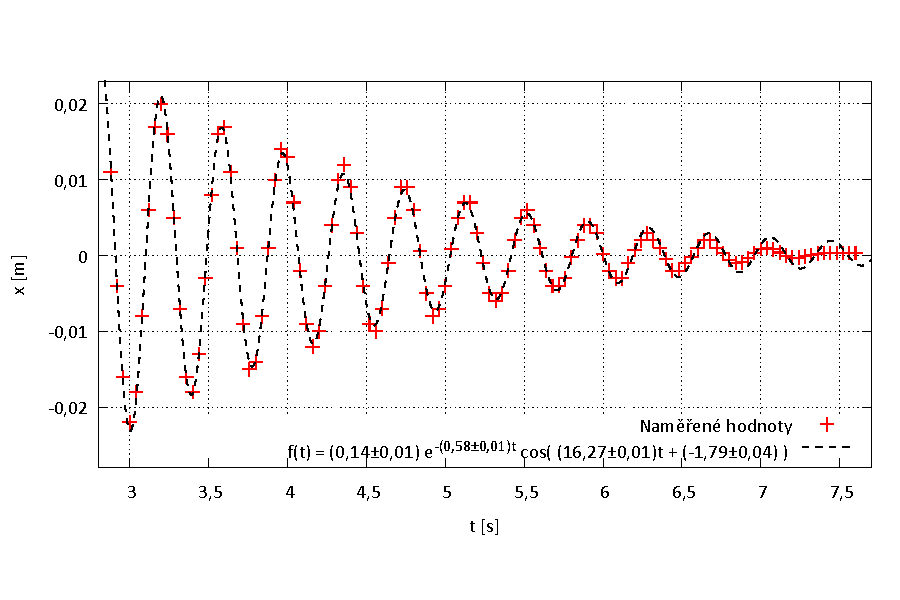
\includegraphics[width=\linewidth]{../gnuplot/10_lho_tlum_20g_2.pdf}
	    \vspace*{-2cm}
			\caption{Graf časového průběhu tlumených kmitů LHO pro závaží o hmotnosti $m=20$ g; $x$ je poloha v závislosti na čase $t$. Naměřené hodnoty jsme proložili podle rovnice (\ref{eq:fit_tlum}).}
			\label{fig:lho_tlum_20g}
	\end{center}
	\end{figure}
	
	\begin{figure}[h!]
	\begin{center}
		\vspace*{-1cm}
		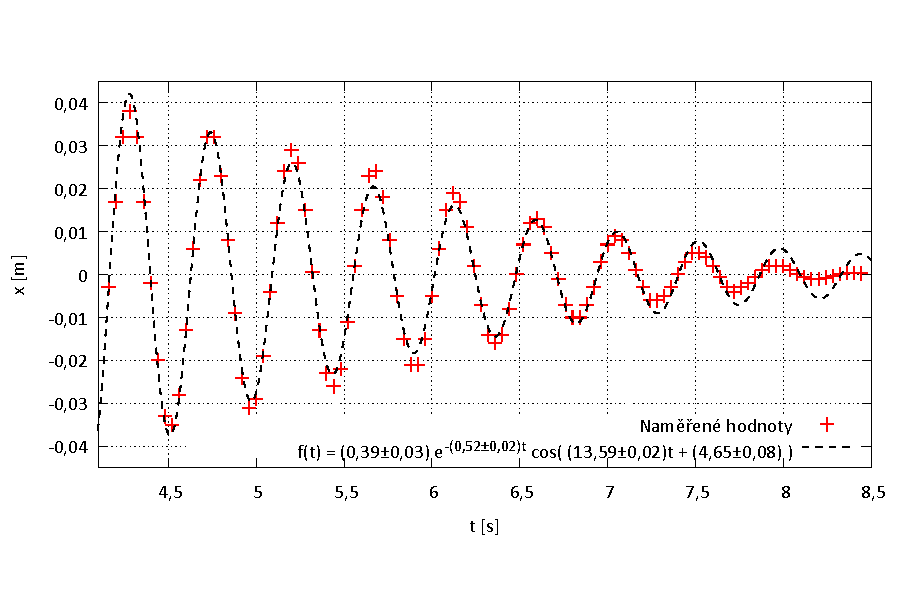
\includegraphics[width=\linewidth]{../gnuplot/10_lho_tlum_40g_2.pdf}
		\vspace*{-2cm}    
		\caption{Graf časového průběhu tlumených kmitů LHO pro závaží o hmotnosti $m=40$ g; $x$ je poloha v závislosti na čase $t$. Naměřené hodnoty jsme proložili podle rovnice (\ref{eq:fit_tlum}).}
		\label{fig:lho_tlum_40g}
	\end{center}
	\end{figure}
	
	\begin{figure}[h]
	\begin{center}
	\vspace*{-1cm}
		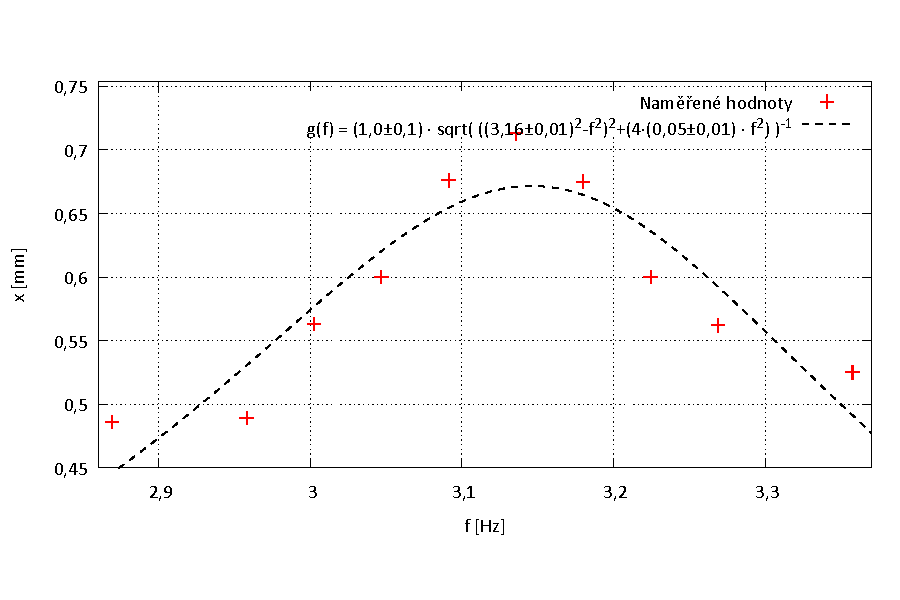
\includegraphics[width=\linewidth]{../gnuplot/10_lho_rezonance_20g.pdf}
	\vspace*{-2cm}
			\caption{Graf závislosti maximální amplitudy $x$ na frekvenci $f$ budící síly v okolí rezonance pro závaží o hmotnosti $m=20$ g. Naměřené hodnoty jsme proložili podle rovnice (\ref{eq:fit_rezonance}).}
			\label{fig:lho_rezo_20g}
	\end{center}
	\end{figure}
	
	\begin{figure}[h!]
	\begin{center}
		\vspace*{-1cm}
		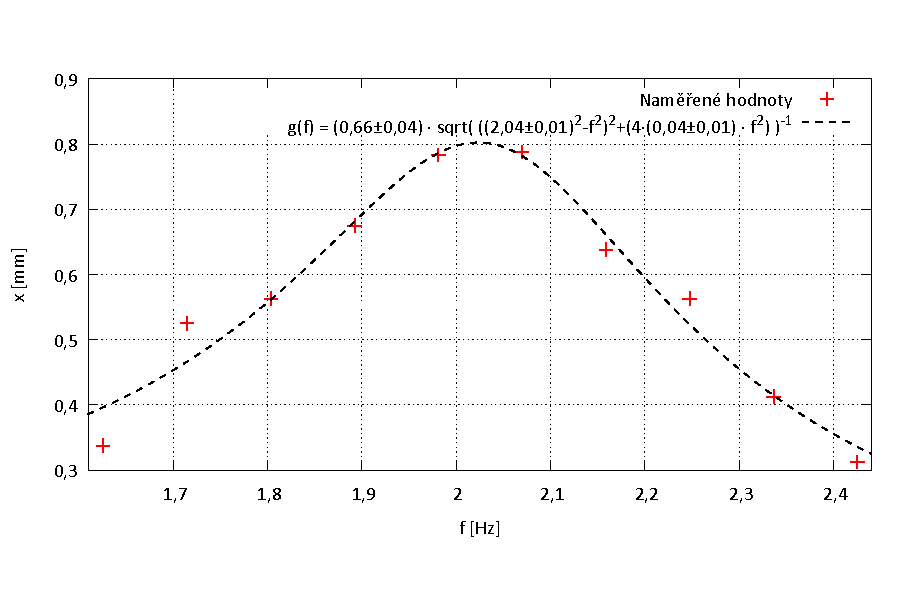
\includegraphics[width=\linewidth]{../gnuplot/10_lho_rezonance_40g.pdf}
	\vspace*{-2cm}
			\caption{Graf závislosti maximální amplitudy $x$ na frekvenci $f$ budící síly v okolí rezonance pro závaží o hmotnosti $m=40$ g. Naměřené hodnoty jsme proložili podle rovnice (\ref{eq:fit_rezonance}).}
			\label{fig:lho_rezo_40g}
	\end{center}
	\end{figure}
		
	\begin{figure}[h]
	\begin{center}
	\vspace*{-1cm}
		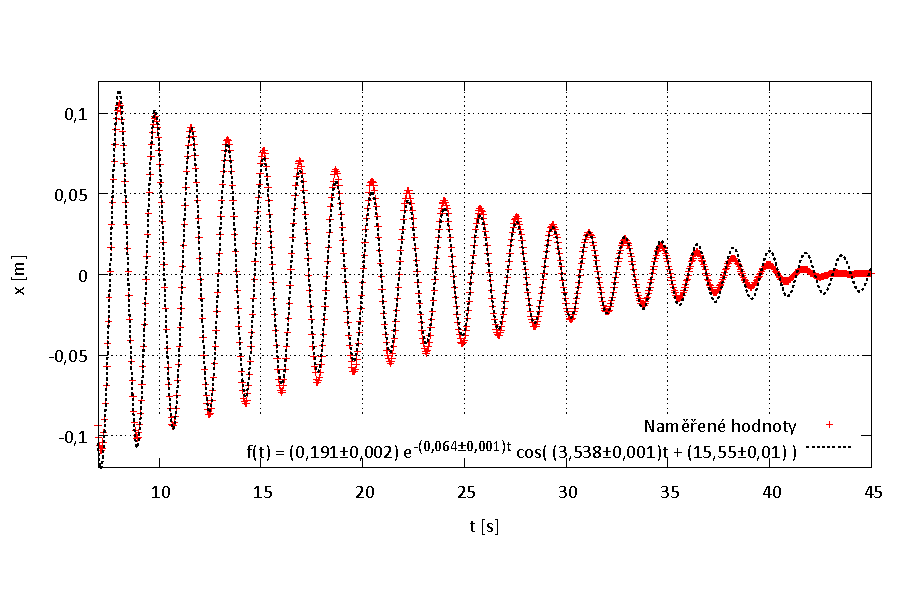
\includegraphics[width=\linewidth]{../gnuplot/10_pohl_tlum_10g_2.pdf}
	\vspace*{-2cm}
			\caption{Graf časového průběhu netlumených kmitů Pohlova kyvadla pro závaží o hmotnosti $m=10$ g; $x$ je poloha v závislosti na čase $t$. Naměřené hodnoty jsme proložili podle rovnice (\ref{eq:fit_tlum}).}
			\label{fig:pohl_tlum_10g}
	\end{center}
	\end{figure}

	\begin{figure}[h!]
	\begin{center}
	\vspace*{-1cm}
		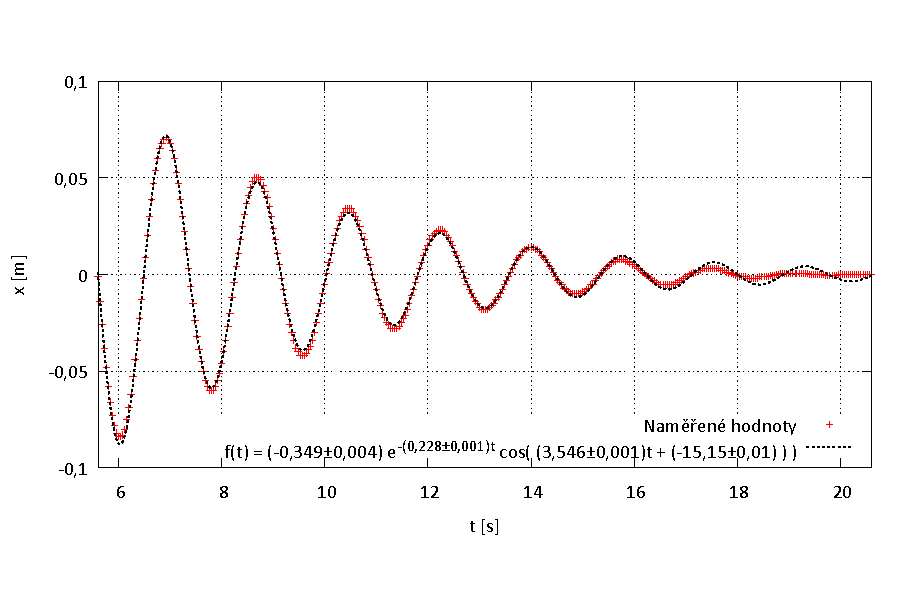
\includegraphics[width=\linewidth]{../gnuplot/10_pohl_dekr_04_10g.pdf}
	\vspace*{-2cm}
			\caption{Graf časového průběhu tlumených kmitů Pohlova kyvadla pro závaží o hmotnosti $m=10$ g a tlumícího proudu $I = 0,4$ A; $x$ je poloha v závislosti na čase $t$. Naměřené hodnoty jsme proložili podle rovnice (\ref{eq:fit_tlum}).}
			\label{fig:pohl_dekr_04}
	\end{center}
	\end{figure}

	\begin{figure}[h]
	\begin{center}
	\vspace*{-1cm}
		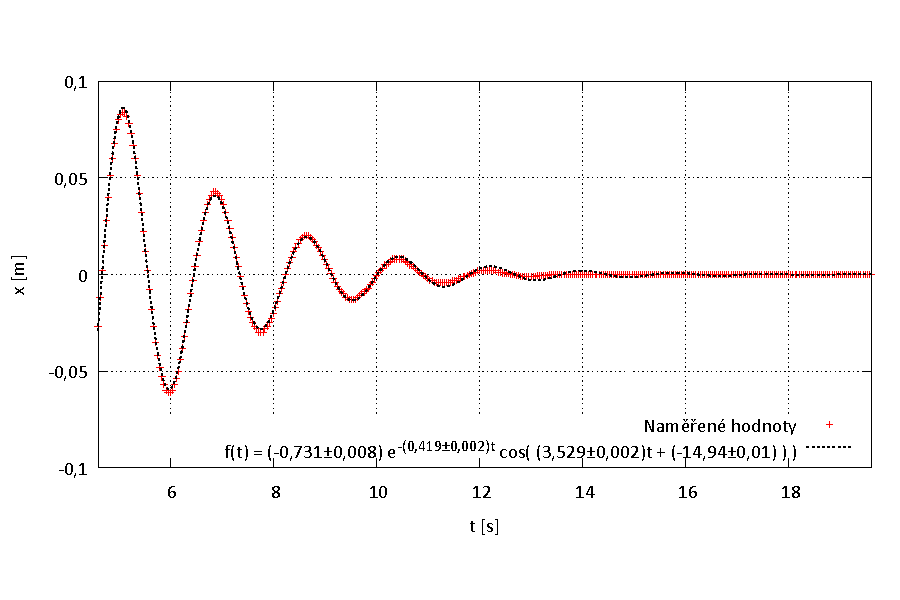
\includegraphics[width=\linewidth]{../gnuplot/10_pohl_dekr_06_10g.pdf}
	\vspace*{-2cm}
			\caption{Graf časového průběhu tlumených kmitů Pohlova kyvadla pro závaží o hmotnosti $m=10$ g a tlumícího proudu $I = 0,6$ A; $x$ je poloha v závislosti na čase $t$. Naměřené hodnoty jsme proložili podle rovnice (\ref{eq:fit_tlum}).}
			\label{fig:pohl_dekr_06}
	\end{center}
	\end{figure}

	\begin{figure}[h!]
	\begin{center}
	\vspace*{-1cm}
		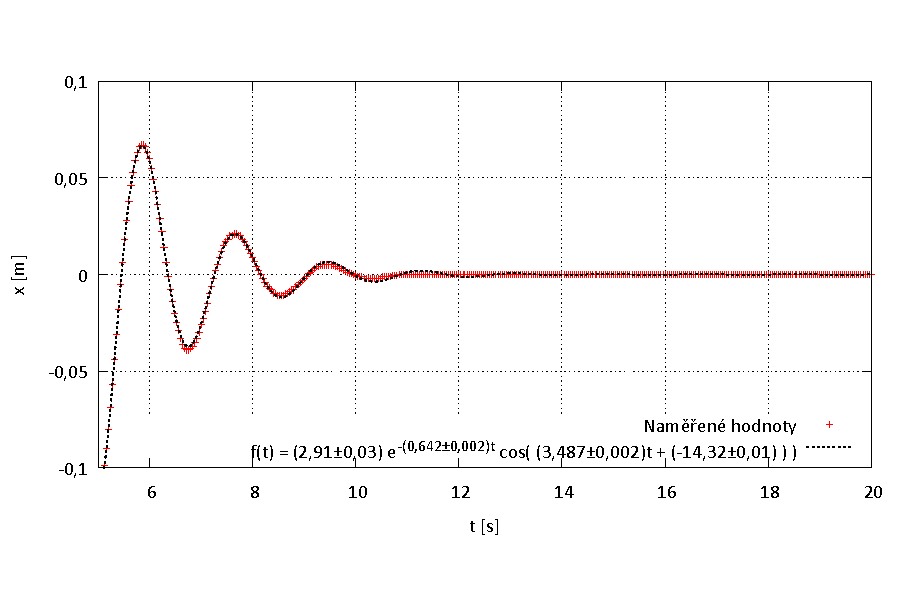
\includegraphics[width=\linewidth]{../gnuplot/10_pohl_dekr_08_10g.pdf}
	\vspace*{-2cm}
			\caption{Graf časového průběhu tlumených kmitů Pohlova kyvadla pro závaží o hmotnosti $m=10$ g a tlumícího proudu $I = 0,8$ A; $x$ je poloha v závislosti na čase $t$. Naměřené hodnoty jsme proložili podle rovnice (\ref{eq:fit_tlum}).}
			\label{fig:pohl_dekr_08}
	\end{center}
	\end{figure}			

	\begin{figure}[h]
	\begin{center}
	\vspace*{-1cm}
		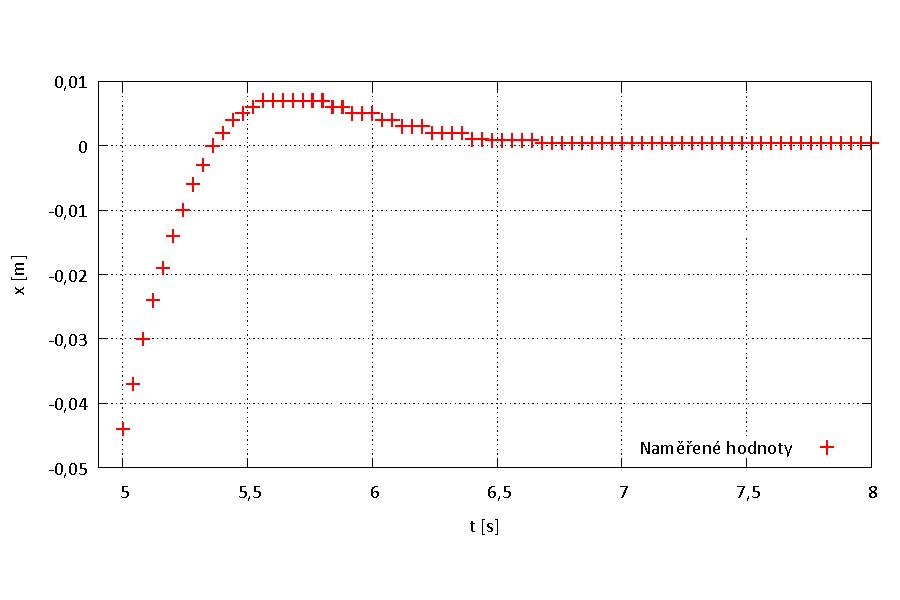
\includegraphics[width=\linewidth]{../gnuplot/10_pohl_dekr_16_10g.pdf}
	\vspace*{-2cm}
			\caption{Graf časového průběhu tlumených kmitů Pohlova kyvadla pro závaží o hmotnosti $m=10$ g a tlumícího proudu $I = 1,5$ A; $x$ je poloha v závislosti na čase $t$.}
			\label{fig:pohl_dekr_16}
	\end{center}
	\end{figure}
	
	\begin{figure}[h!]
	\begin{center}
	\vspace*{-1cm}
		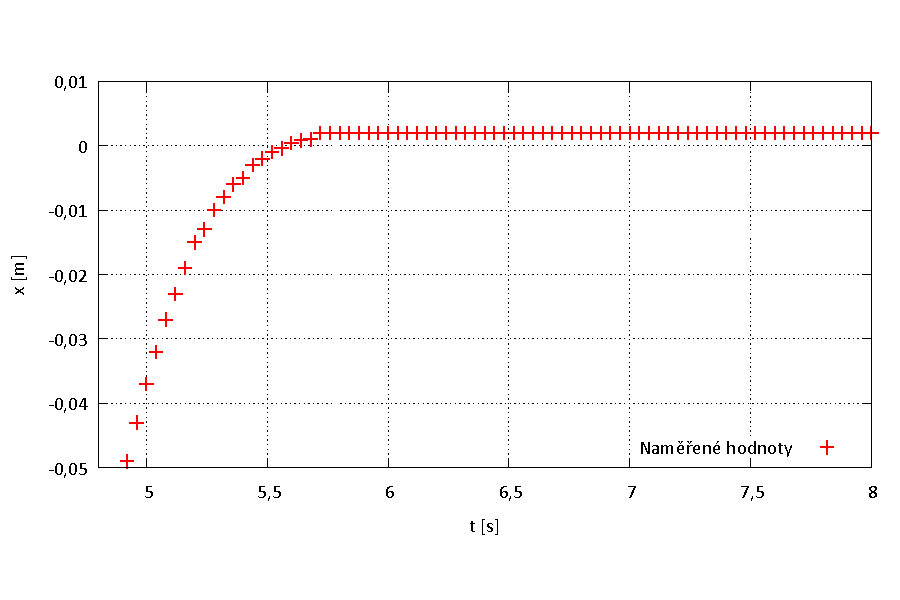
\includegraphics[width=\linewidth]{../gnuplot/10_pohl_dekr_18_10g.pdf}
	\vspace*{-2cm}
			\caption{Graf časového průběhu tlumených kmitů Pohlova kyvadla pro závaží o hmotnosti $m=10$ g a tlumícího proudu $I = 1,8$ A; $x$ je poloha v závislosti na čase $t$.}
			\label{fig:pohl_dekr_18}
	\end{center}
	\end{figure}
	
	\begin{figure}[h]
	\begin{center}
	\vspace*{-1cm}
		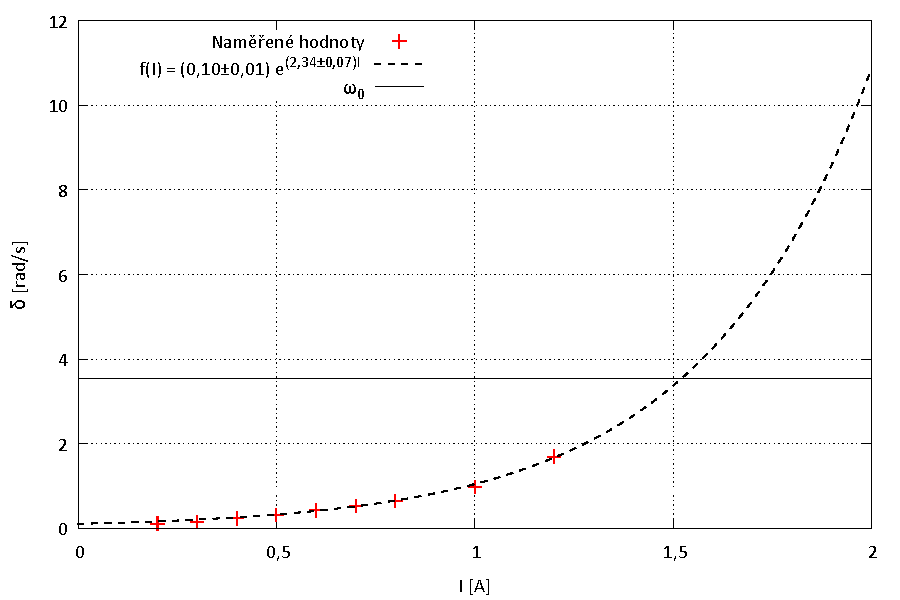
\includegraphics[width=\linewidth]{../gnuplot/10_pohl_dekrementy.pdf}
	\vspace*{-1cm}
			\caption{Graf závislosti dekrementu útlumu $\delta$ na velikosti tlumícího proudu $I$ na cívkách Pohlova kyvadla. Naměřené hodnoty jsme proložili odpovídající funkcí.}
			\label{fig:pohl_dekrementy}
	\end{center}
	\end{figure}						
	
% --- Konec dokumentu --------------------------------------------------


\end{document}

